\section{Hypothesis Tests}

\subsection{Fisher's Null Hypothesis Test}

\begin{frame}{Fisher's Null Hypothesis Test}

\structb{Overview.}
\begin{enumerate}
	\justifying
	\item Set up a \highlightg{null hypothesis} $H_0$ that compares a population para-meter $\theta$ to a given null value $\theta_0$.
	\begin{itemize}
		\item $H_0: \theta = \theta_0$,
		\item $H_0: \theta \leq \theta_0$,
		\item $H_0: \theta \geq \theta_0$.
	\end{itemize}
	\item Try to reject the null hypothesis by finding \highlightg{P-value} for the test.\\
	\begin{itemize}
		\justifying
		\item \underline{One-tailed}: upper bound of probability of obtaining the data or more extreme data (based on the null hypothesis), given that the null hypothesis is true.
		\begin{align*}
		P[D|H_0]\leq P\U{-value}.
		\end{align*}
		\item \underline{Two-tailed}: twice of p-value for one-tailed test.
	\end{itemize}
	\item We either 
	\begin{itemize}
		\item fail to reject $H_0$ or
		\item reject $H_0$ at the [p-value] level of significance.
	\end{itemize}
\end{enumerate}

\end{frame}

\begin{frame}{One-tailed Test}

\justifying
\structb{Null hypothesis.}
\begin{align*}
H_0: \theta \leq \theta_0 \qquad \U{or} \qquad H_0: \theta \geq \theta_0.
\end{align*}
\structb{Test for mean.} Suppose the sample mean $\overline{X}$ follows a normal distribution with mean $\mu$.
\begin{figure}[htbp]
	\centering
	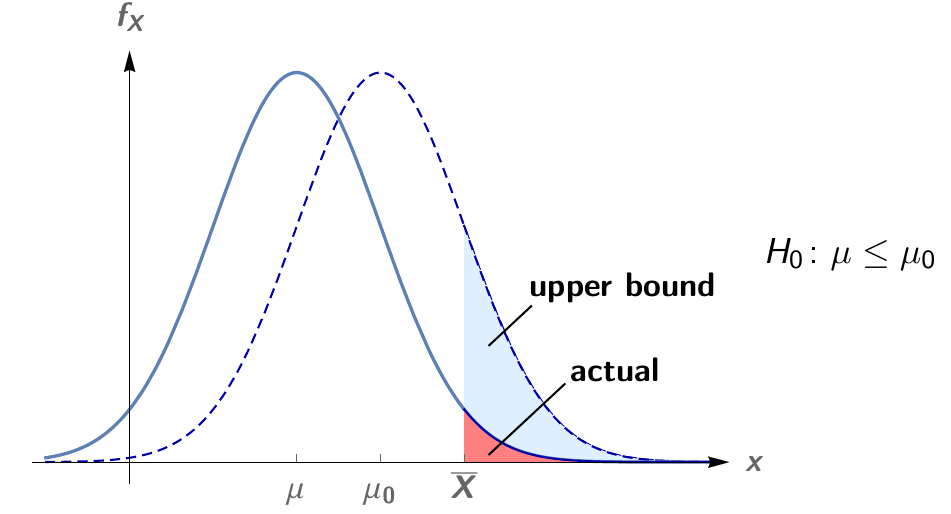
\includegraphics[width=8cm]{./images/rc5fig1.png}
\end{figure}

\end{frame}

\begin{frame}{Two-tailed Test}

\justifying
\structb{Null hypothesis.}
\begin{align*}
H_0: \theta = \theta_0.
\end{align*}
\structb{Test for mean.} Suppose the sample mean $\overline{X}$ follows a normal distribution with mean $\mu$.
\begin{figure}[htbp]
	\centering
	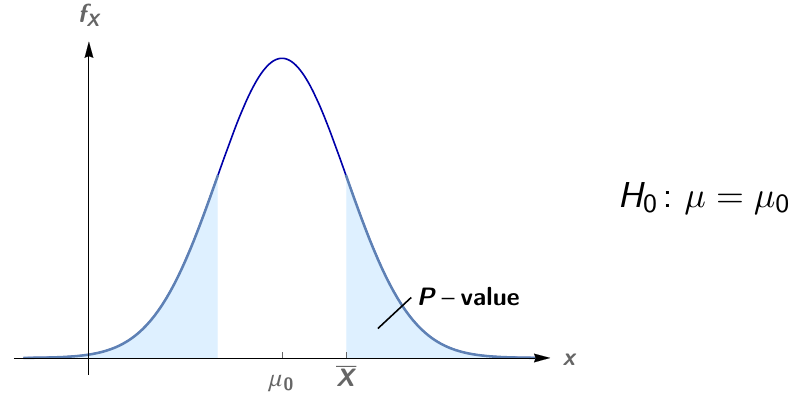
\includegraphics[width=8cm]{./images/rc5fig2.png}
\end{figure}

\end{frame}


\subsection{Neyman-Pearson Decision Theory}

\begin{frame}{Neyman-Pearson Decision Theory}

\structb{Overview.}
\begin{enumerate}
	\justifying
	\item Set up a \highlightg{null hypothesis} $H_0$ and an \highlightg{alternative hypothesis} $H_1$.
	\item Determine a desirable $\alpha$ and $\beta$, where
	\begin{itemize}
		\item $\alpha := P[\U{reject\ } H_0|H_0 \U{\ true}]$,
		\item $\beta := P[\U{accept\ } H_0|H_1 \U{\ true}]$, and
		\item $\U{power} := 1 - \beta = P[\U{reject\ } H_0|H_1 \U{\ true}]$.
	\end{itemize}
	\item Use $\alpha$ and $\beta$ to determine the appropriate sample size $n$. \highlightr{$\Delta$}
	\item Use $\alpha$ and $n$ to determine the critical region. \highlightr{$\Delta$}
	\item Obtain sample statistics, and reject $H_0$ at significance level $\alpha$ and accept $H_1$ if the test statistic falls into critical region. Otherwise, accept $H_0$.
\end{enumerate}

\end{frame}

\begin{frame}{Choosing the Sample Size}

\justifying
\structb{Normal case.} Suppose the sample mean $\overline{X}$ follows a normal distri-bution with unknown mean $\mu$ and known variance $\sigma^2$, and we have hypothesis
\begin{align*}
H_0: \mu = \mu_0, \qquad H_1: |\mu - \mu_0| \geq \delta_0.
\end{align*}\\
\only<1>{
	\structb{Relation between $\alpha$, $\beta$ $\delta$, $\sigma$ and $n$.} With true mean $\mu = \mu_0 + \delta$, the test statistic $Z = \dfrac{\overline{X} - \mu_0}{\sigma/\sqrt{n}}\sim\U{N}(\delta\sqrt{n}/\sigma, 1)$.
	\begin{align*}
	P[\U{fail\ to\ reject\ } H_0|\mu = \mu_0 + \delta] & = \frac{1}{\sqrt{2\pi}}\int_{-z_{\alpha/2}}^{z_{\alpha/2}} e^{-(t-\delta\sqrt{n}/\sigma)^2/2} \U{d}t \\
	& = \frac{1}{\sqrt{2\pi}}\int_{-z_{\alpha/2}-\delta\sqrt{n}/\sigma}^{z_{\alpha/2}-\delta\sqrt{n}/\sigma} e^{-t^2/2}\U{d}t \\
	& \approx \frac{1}{\sqrt{2\pi}} \int_{-\infty}^{z_{\alpha/2}-\delta\sqrt{n}/\sigma} e^{-t^2/2}\U{d}t \overset{!}{=} \beta,
	\end{align*}
	where we set $-z_{\beta} = z_{\alpha/2}-\delta\sqrt{n}/\sigma$.
}
\uncover<2>{
	\structb{Choosing the sample size $n$.}
	\begin{align*}
	n\approx \frac{(z_{\alpha/2} + z_{\beta})^2\sigma^2}{\delta^2},
	\end{align*}
	where $z_{\alpha/2}$ and $z_{\beta}$ satisfies that
	\begin{align*}
	\Phi(z_{\alpha/2}) = 1 - \alpha/2, \qquad \Phi(z_{\beta}) = 1 - \beta,
	\end{align*}
	given cumulative distribution function $\Phi$ of standard normal distribution.
}

\end{frame}


\begin{frame}{Choosing the Sample Size}

\structb{Normal case.}
\begin{figure}[htbp]
	\centering
	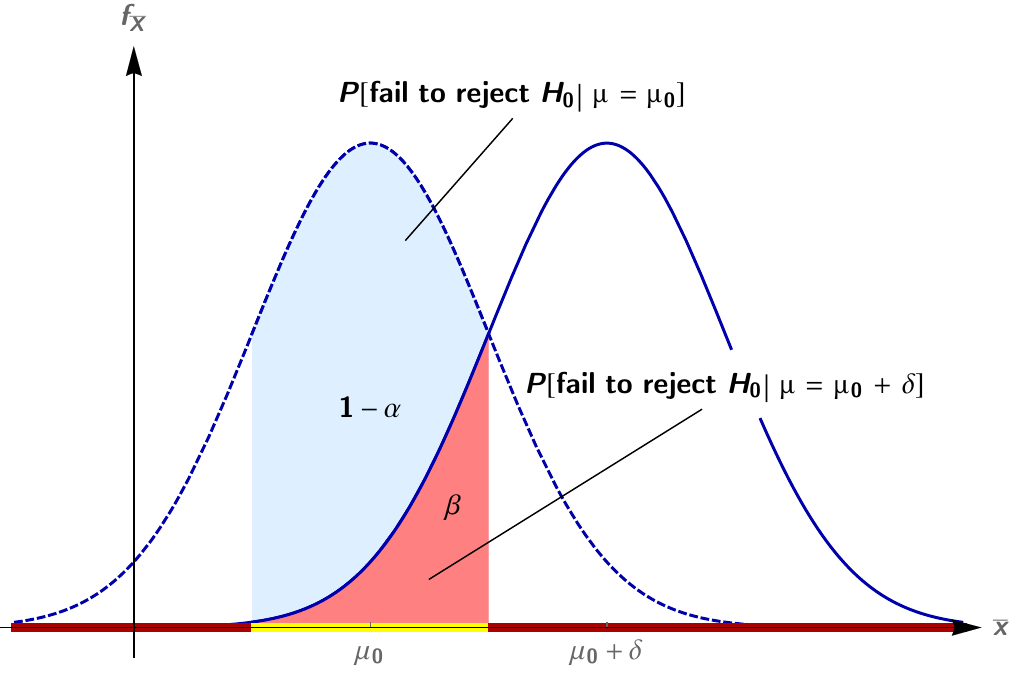
\includegraphics[width=8cm]{./images/rc5fig5.png}
\end{figure}

\end{frame}


\begin{frame}{Choosing the Sample Size}

\structb{More general case: OC curve.}
\begin{enumerate}
	\justifying
	\item For normal test, calculate
	\begin{align*}
	d := \frac{|\mu - \mu_0|}{\sigma}.
	\end{align*}
	\highlightr{Note.} The abscissa might change corresponding to the distri-bution of test.
	\item Look up in OC curve for sample size $n$.
\end{enumerate}

\end{frame}


\begin{frame}{Choosing the Sample Size}

\structb{More general case: OC curve.}
\begin{figure}[htbp]
	\centering
	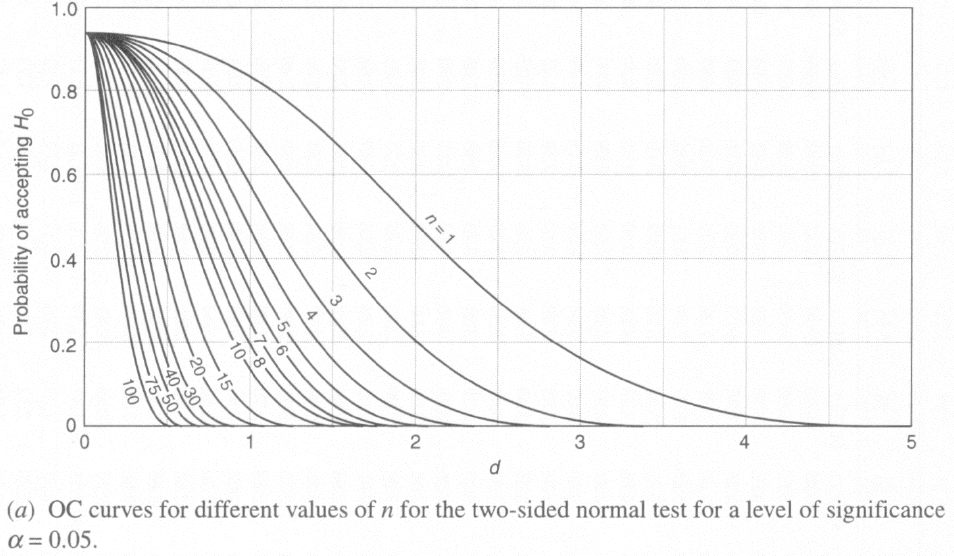
\includegraphics[width=\linewidth]{./images/rc5fig3.png}
\end{figure}

\end{frame}


\begin{frame}{Choosing the Sample Size}

\structb{More general case: OC curve.}
\begin{figure}[htbp]
	\centering
	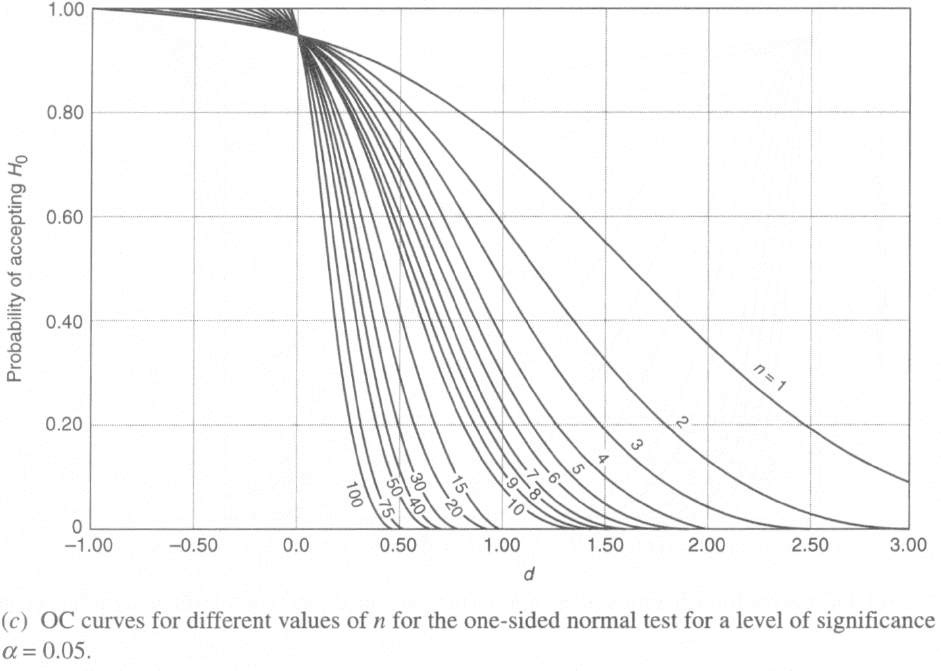
\includegraphics[width=\linewidth]{./images/rc5fig4.png}
\end{figure}

\end{frame}


\begin{frame}{Choosing the Critical Region}

\justifying
\structb{Determine the critical region using $\alpha$ and $n$.} The \highlightg{critical region} is chosen so that if $H_0$ is true, then the probability of test statistic's value falling into the critical region is no more than $\alpha$. \\
\structb{Critical region for mean.} Suppose the sample mean $\overline{X}$ follows a normal distribution with unknown mean $\mu$ and known variance $\sigma^2$, with $H_0: \mu = \mu_0$. Then the test statistic
\begin{align*}
Z = \frac{\overline{X} - \mu_0}{\sigma/\sqrt{n}} \sim \U{N}(0, 1),
\end{align*}
and thus the critical region is obtained from
\begin{align*}
\frac{|\overline{X} - \mu_0|}{\sigma/\sqrt{n}} > z_{\alpha/2}.
\end{align*}
We reject $H_0$ at significance level $\alpha$ and accept $H_1$ if $\overline{X}$ falls in this critical region.

\end{frame}

\begin{frame}{Neyman-Pearson Decision Theory}

\justifying
\structb{Example (assignment 5.3).} (... long description ...) ... a researcher would like to test the hypotheses 
\begin{align*}
H_0: \mu \leq 4\U{\ hours}, \qquad H_1: \mu \geq 4.5\U{\ hours}.
\end{align*}
A random sample of 50 battery packs is selected and subjected to a life test. Assume that the battery life is normally distributed with standard deviation $\sigma = 0.2$ hours.
\only<2>{
	\begin{itemize}
		\justifying
		\item[(i)] Using the sample mean life span $\overline{X}$ as a test statistic, what is the critical region if $\alpha = 5\%$ is desired.
		\begin{align*}
		\frac{\overline{X} - \mu_0}{\sigma/\sqrt{n}} > z_{\alpha} \quad \Rightarrow\quad \overline{X} > \mu_0 + z_{\alpha}\frac{\sigma}{\sqrt{n}} =: L_l.
		\end{align*}
	\end{itemize}
}
\only<3>{
	\begin{itemize}
		\justifying
		\item[(ii)] Find the power of the test, i.e., the probability of rejecting $H_0$ if $H_1$ is true.
		\begin{align*}
		\U{power} & = P[\overline{X} > L_l | \mu\geq 4.5, \sigma=0.2] \\
		& \geq P[\overline{X} > L_l|\mu=4.5, \sigma=0.2] \\
		& = P\left[\frac{\overline{X} - 4.5}{\sigma/\sqrt{n}} > \frac{L_l-4.5}{\sigma/\sqrt{n}} \right].
		\end{align*}
	\end{itemize}
}
\only<4>{
	\begin{itemize}
		\justifying
		\item[(iii)] What sample size would be required to obtain a power of at least 0.97?
		\begin{align*}
		& \alpha = 0.05, \qquad \beta = 1 - 0.97 = 0.03, \qquad \delta = 0.5 \\
		\Rightarrow & n \approx \frac{(z_{\alpha} + z_{\beta})^2\sigma^2}{\delta^2}.
		\end{align*}
	\end{itemize}
}
\uncover<5>{
	\begin{itemize}
		\justifying
		\item[(iv)] The sample mean life span turns out to be $\overline{x} = 4.05$ hours. Is $H_0$ rejected? Find a confidence interval for $\mu$. \\~\\
		Since $\overline{x} > L_l$, $H_0$ is rejected. A 95\% confidence interval for $\mu$ is given by
		\begin{align*}
		\mu \geq \overline{x} - z_{\alpha}\frac{\sigma}{\sqrt{n}}.
		\end{align*}
	\end{itemize}
}


\end{frame}

\begin{frame}{Confidence Interval vs. Critical Region}

\justifying
Suppose we would like to estimate the mean $\mu$ of a sample $X_1, \ldots, X_n$ of size $n$.
\begin{itemize}
	\justifying
	\item \structb{Confidence interval.} Given a sample data with specific values, the CI gives an interval for the unknown mean $\mu$.
	\item \structb{Critical region.} Given a null value $\mu_0$, the critical region gives an interval for sample mean $\overline{X}$ before obtaining specific values.
	\item \structb{Relation.} The null hypothesis $H_0$ is rejected $\Leftrightarrow$ $\overline{X}$ lies in the critical region $\Leftrightarrow$ null value $\mu_0$ lies outside the confidence interval.
\end{itemize}


\end{frame}


\subsection{Difficulties of Designing a Proper Hypothesis Test}

\begin{frame}{Tossing a Coin}

\justifying
\structb{Setup.} Suppose we have coin, without knowing whether it is fair or not. Let the probability of head be $p$ for the Bernoulli random variable, and we wish to test the hypotheses
\begin{align*}
H_0: p \leq p_0, \qquad H_1: p > p_0.
\end{align*}
\structb{Discussion.} Following the discussion above, we might toss the coin for $n$ times, and gather a set of sample $X_1, \ldots, X_n$, where each $X_i$ is a Bernoulli random variable. Let $\displaystyle Y = \sum_{i=1}^n X_i$. Given a desired significance level $\alpha$, let $y_{\alpha} \in \N$ such that
\footnotesize
\begin{align*}
Pr[Y\geq y_{\alpha}|p=p_0] & = \sum_{y=y_{\alpha}}^n \binom{n}{y} p_0^{y}(1-p_0)^{n-y} \leq \alpha, \\
Pr[Y\geq y_{\alpha}-1|p=p_0] & = \sum_{y=y_{\alpha}-1}^n \binom{n}{y} p_0^{y}(1-p_0)^{n-y} > \alpha.
\end{align*}
\normalsize
Then we would reject $H_0$ at significance level $\alpha$ if $Y \geq y_{\alpha}$.

\end{frame}


\begin{frame}{Tossing a Coin}

\justifying
\structb{Setup (with prior).} Suppose we have coin, without knowing whether it is fair or not. Let the probability of head be $p$ for the Bernoulli random variable, and we wish to test the hypotheses
\begin{align*}
H_0: p \leq p_0, \qquad H_1: p > p_0.
\end{align*}
Now suppose we have an additional prior information. It is learned from the factory which is producing this type of coin that the para-meter $p$ follows a Beta distribution with density function
\begin{align*}
f_P(p) = \frac{\Gamma(\alpha + \beta)}{\Gamma(\alpha)\Gamma(\beta)}p^{\alpha-1}(1 - p)^{\beta-1}, \qquad p\in (0, 1),
\end{align*}
where $\alpha = 7,\beta = 2$. Assume we want to test the hypothesis when the null value $p_0 = 0.5$.

\end{frame}

\begin{frame}{Tossing a Coin}

\justifying
\structb{Setup.} 
\begin{figure}[htbp]
	\centering
	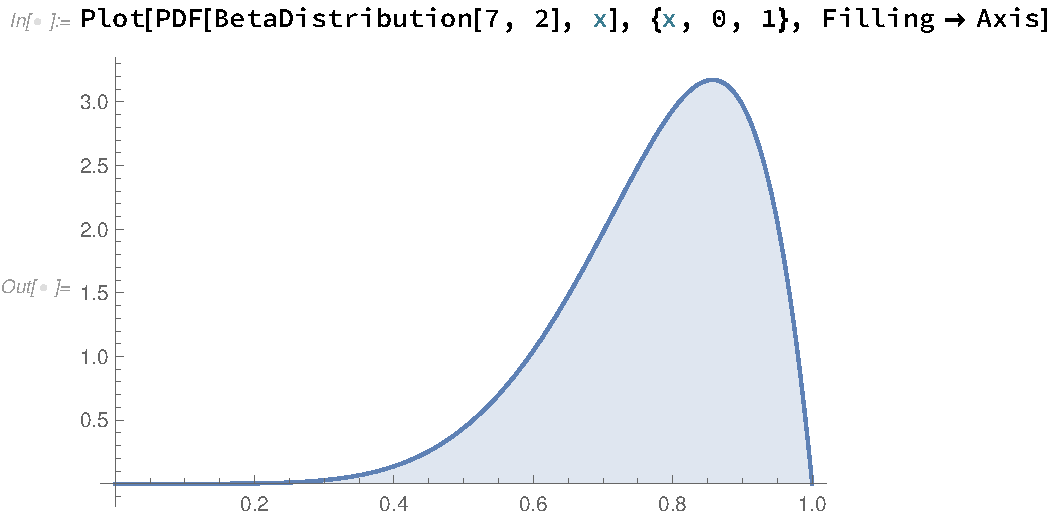
\includegraphics[width=\linewidth]{./images/rc5fig6.pdf}
\end{figure}

\end{frame}


\begin{frame}{Tossing a Coin}

\justifying
\structb{Bayesian analysis.} We have Bayes's theorem (for density function)
\begin{align*}
P[A|B] = \frac{P[B|A]\cdot P[A]}{P[B]} = \frac{P[B, A]}{P[B]}.
\end{align*}
Then in terms of cumulative distribution function, with $\varepsilon > 0$,
\begin{align*}
F_{Y|X}(y|x) & = \lim_{\varepsilon \rightarrow 0} P[Y\leq y|x < X \leq x + \varepsilon] \\
& = \lim_{\varepsilon \rightarrow 0} \frac{P[Y\leq y, x < X \leq x + \varepsilon]}{P[x < X \leq x + \varepsilon]} \\
& = \lim_{\varepsilon \rightarrow 0} \frac{F_{XY}(x + \varepsilon, y) - F_{XY}(x, y)}{F_X(x+\varepsilon) - F_X(x)} = \frac{1}{f_X(x)}\frac{\partial F_{XY}(x, y)}{\partial x}. \\
\Rightarrow f_{Y|X}(y|x) & = \frac{\partial F_{Y|X}(y|x)}{\partial y} = \frac{f_{XY}(x, y)}{f_X(x)} \propto f_{X|Y}(x|y) f_Y(y).
\end{align*}

\end{frame}


\begin{frame}{Tossing a Coin}

\justifying
\structb{Bayesian analysis.} With this additional prior information, according to Bayes's theorem, it is more appropriate to calculate
\begin{align*}
f_{P|Y}(p|y) & \propto f_{Y|P}(y|p)f_P(p) \\
& \propto \binom{n}{y} p^y(1-p)^{n-y} \cdot\frac{\Gamma(\alpha + \beta)}{\Gamma(\alpha)\Gamma(\beta)}p^{\alpha-1}(1 - p)^{\beta-1} \\
& \propto p^{y+\alpha-1} (1-p)^{n-y+\beta-1}.
\end{align*}
and thus
\begin{align*}
f_{P|Y}(p|y) = \frac{\Gamma(\alpha' + \beta')}{\Gamma(\alpha')\Gamma(\beta')}p^{\alpha'-1}(1 - p)^{\beta'-1},
\end{align*}
where $\alpha' = y + \alpha, \beta' = n - y + \beta$.

\end{frame}

\begin{frame}{Tossing a Coin}

\justifying
\structb{Bayesian analysis.} Then we are able to calculate $P[H_0|D]$, which we are really interested in, as
\begin{align*}
P[H_0|D] = F_{P|Y}(p_0|y) = \int_0^{p_0} f_{P|Y}(p|y) \U{d}p.
\end{align*}
Let $y_{\alpha}$ satisfies that
\begin{align*}
1 - F_{P|Y}(p|y_{\alpha}) & = 1 - \int_0^{p_{0}} f_{P|Y}(p|y_{\alpha}) \U{d}p \leq \alpha,\\
1 - F_{P|Y}(p|y_{\alpha}-1) & = 1 - \int_0^{p_{0}} f_{P|Y}(p|y_{\alpha}) \U{d}p > \alpha.
\end{align*}
Then finally we would reject $H_0: p\leq p_0$ if $Y\geq y_{\alpha}$. 

\end{frame}


\section{Test for Statistics}

\subsection{Single Sample Tests for Mean and Variance}

\begin{frame}{Test for Mean (Variance Known)}

\justifying
\structb{Z-test.} Let $X_1, \ldots, X_n$ be a random sample of size $n$ from a normal distribution with \highlightr{unknown} mean $\mu$ and \highlightr{known} variance $\sigma^2$. Let $\mu_0$ be a null value of the mean. Then the test statistic is given by
\begin{align*}
Z = \frac{\overline{X} - \mu_0}{\sigma/\sqrt{n}}.
\end{align*}
We reject at significance level $\alpha$
\begin{itemize}
	\item $H_0: \mu = \mu_0$ if $|Z| > z_{\alpha/2}$,
	\item $H_0: \mu\leq \mu_0$ if $Z > z_{\alpha}$,
	\item $H_0: \mu\geq \mu_0$ if $Z < -z_{\alpha}$.
\end{itemize}
\structb{OC curve.} The abscissa is defined by
\begin{align*}
d = \frac{|\mu - \mu_0|}{\sigma}.
\end{align*}

\end{frame}


\begin{frame}{Test for Mean (Variance Unknown)}

\justifying
\structb{T-test.} Let $X_1, \ldots, X_n$ be a random sample of size $n$ from a normal distribution with \highlightr{unknown} mean $\mu$ and \highlightr{unknown} variance $\sigma^2$. Let $\mu_0$ be a null value of the mean. Then the test statistic is given by
\begin{align*}
T_{n-1} = \frac{\overline{X} - \mu_0}{S/\sqrt{n}}.
\end{align*}
We reject at significance level $\alpha$
\begin{itemize}
	\item $H_0: \mu = \mu_0$ if $|T_{n-1}| > t_{\alpha/2, n-1}$,
	\item $H_0: \mu\leq \mu_0$ if $T_{n-1} > t_{\alpha, n-1}$,
	\item $H_0: \mu\geq \mu_0$ if $T_{n-1} < -t_{\alpha, n-1}$.
\end{itemize}
\structb{OC curve.} The abscissa is defined by
\begin{align*}
d = \frac{|\mu - \mu_0|}{\sigma},
\end{align*}
where in practice, the unknown $\sigma$ can be substituted by $S$.

\end{frame}

\begin{frame}{Test for Variance}

\justifying
\structb{Chi-squared test.} Let $X_1, \ldots, X_n$ be a random sample of size $n$ from a normal distribution with unknown variance $\sigma^2$. Let $\sigma^2_0$ be a null value of the variance. Then the test statistic is given by
\begin{align*}
\chi_{n-1}^2 = \frac{(n-1)S^2}{\sigma_0^2}.
\end{align*}
We reject at significance level $\alpha$
\begin{itemize}
	\item $H_0: \sigma = \sigma_0$ if $\chi_{n-1}^2 \in (0, \chi_{1-\alpha/2, n-1}^2) \cup (\chi_{\alpha/2, n-1}^2, \infty)$,
	\item $H_0: \sigma\leq \sigma_0$ if $\chi_{n-1}^2 > \chi_{\alpha, n-1}^2$,
	\item $H_0: \sigma\geq \sigma_0$ if $\chi_{n-1}^2 < \chi_{1-\alpha, n-1}^2$.
\end{itemize}
\structb{OC curve.} The abscissa is defined by
\begin{align*}
\lambda = \frac{\sigma}{\sigma_0}.
\end{align*}

\end{frame}


\subsection{Non-Parametric Single Sample Tests for Median}

\begin{frame}{Sign Test for Median}

\justifying
\structb{Sign test.} Let $X_1, \ldots, X_n$ be a random sample of size $n$ from an arbitrary continuous distribution and let 
\begin{align*}
Q_{+} = \#\{X_k: X_k - M_0 > 0\}, \qquad Q_{-} = \#\{X_k: X_k - M_0 < 0\}.
\end{align*}
We reject at a significance level $\alpha$
\begin{itemize}
	\justifying
	\item $H_0: M\leq M_0$ if $P[Y\leq q_-|M = M_0] < \alpha$,
	\item $H_0: M\geq M_0$ if $P[Y\leq q_+|M = M_0] < \alpha$,
	\item $H_0: M = M_0$ if $P[Y\leq \min(q_-, q_+)|M = M_0] < \alpha/2$,
\end{itemize}
where $q_-, q_+$ are values of $Q_-, Q_+$, and $Y$ follows a binomial distri-bution with parameters $n'$ and $1/2$, i.e.,
\begin{align*}
P[Y \leq k|M = M_0] = \sum_{y=0}^k \binom{n'}{y} \frac{1}{2^{n'}}, \qquad n' = q_+ + q_-.
\end{align*}

\end{frame}


\begin{frame}{Wilcoxon Signed Rank Test for Median}

\justifying
\structb{Wilcoxon signed rank Test.} Let $X_1, \ldots, X_n$ be a random sample of size $n$ from a \highlightr{symmetric} distribution. Order the $n$ absolute differences $|X_i - M_0|$ according to the magnitude, so that $X_{R_i} - M_0$ is the $R_i$th smallest difference by modulus. If ties in the rank occur, the mean of the ranks is assigned to all equal values. Let
\begin{align*}
W_+ = \sum_{R_i > 0} R_i, \qquad |W_-| = \sum_{R_i < 0} |R_i|.
\end{align*}
We reject at significance level $\alpha$
\begin{itemize}
	\justifying
	\item $H_0: M\leq M_0$ if $|W_-|$ is smaller than the critical value for $\alpha$,
	\item $H_0: M\geq M_0$ if $W_+$ is smaller than the critical value for $\alpha$,
	\item $H_0: M = M_0$ if $W = \min(W_+, |W_-|)$ is smaller than the critical value for $\alpha/2$.
\end{itemize}
As is in the sign test, we use $n'$ after discarding data with $X_i = M_0$.

\end{frame}

\begin{frame}{Wilcoxon Signed Rank Test for Median}

\justifying
\structb{Normal approximation for distribution of $|W_-|$.} Let $I_i$ be the Bernoulli random variable with parameter 1/2 and $I_i = 1$ if $X_i < M_0$. Then we have
\begin{align*}
|W_-| = \sum_{i=1}^n |R_i|I_i \quad\Rightarrow\quad \U{E}[|W_-|] & = \U{E}\left[\sum_{i=1}^n |R_i|I_i \right] \\
& = \sum_{i=1}^n \frac{|R_i|}{2} = \frac{n(n+1)}{4}, \\
\U{Var}|W_-| & = \sum_{i=1}^n |R_i|^2\U{Var}\ I_i \\
& = \sum_{i=1}^n \frac{|R_i|^2}{4} = \frac{n(n+1)(2n+1)}{24}.
\end{align*}


\end{frame}


\begin{frame}{Wilcoxon Signed Rank Test for Median}

\justifying
\structb{Normal approximation for distribution of $|W_-|$ (ties).} Suppose we have a group of $t$ ties, with ranks $R$ and $I$ given by
\begin{align*}
\{R_{j+1}, \ldots, R_{j+t} \}, \qquad \{I_{j+1}, \ldots, I_{j+t} \}.
\end{align*}
Suppose for now $R_j > 0$ and denote
\begin{align*}
\overline{R} = \frac{\sum_{k=1}^t R_{j+k} }{t} = \frac{2R_{j+1} + t - 1}{2} \ \Rightarrow\ R_{j+1} = \overline{R} - \frac{t-1}{2}.
\end{align*}
Since the ranks of ties are calculated as the average of the original ranks, the mean does no change. In terms of variance,
\begin{align*}
& \sum_{k=1}^t |R_{j+k}|^2 \U{Var}\ I_{j+k}-\sum_{k=1}^t |\overline{R}|^2\U{Var}\ I_{j+k} \\
= & \frac{1}{4}\left(\sum_{k=1}^{R_{j+1}+t-1} k^2 - \sum_{k=1}^{R_{j+1}-1}k^2 - t\overline{R}^2\right) =: \frac{1}{4}A.
\end{align*}

\end{frame}


\begin{frame}{Wilcoxon Signed Rank Test for Median}

\justifying
\structb{Normal approximation for distribution of $|W_-|$ (ties).} Then substituting $R_{j+1}$ with $\overline{R}$, we have
\begin{align*}
A & = \frac{\left(a + \dfrac{t}{2}\right)\left(b+\dfrac{t}{2} \right)\left(c + t \right) - \left(a-\dfrac{t}{2} \right)\left(b-\dfrac{t}{2} \right)\left(c-t \right)}{6} - t\overline{R}^2 \\
& = \frac{t^3 - t}{12}.
\end{align*}
where 
\begin{align*}
a = \overline{R} - \frac{1}{2}, \qquad b = \overline{R} + \frac{1}{2}, \qquad c = 2\overline{R}.
\end{align*}
Therefore, for each group of $t$ ties, we need to subtract $(t^3-t)/48$ from the variance. With large sample size, the distribution of $|W_-|$ can be approximated as normal with mean and variance given above. 

\end{frame}


\begin{frame}{Wilcoxon Signed Rank Test for Median}

\justifying
\structb{Critical values for two-tailed test.} For one-tailed test with significance level $\alpha$, use $2\alpha$ for lookup.
\begin{figure}[htbp]
	\centering
	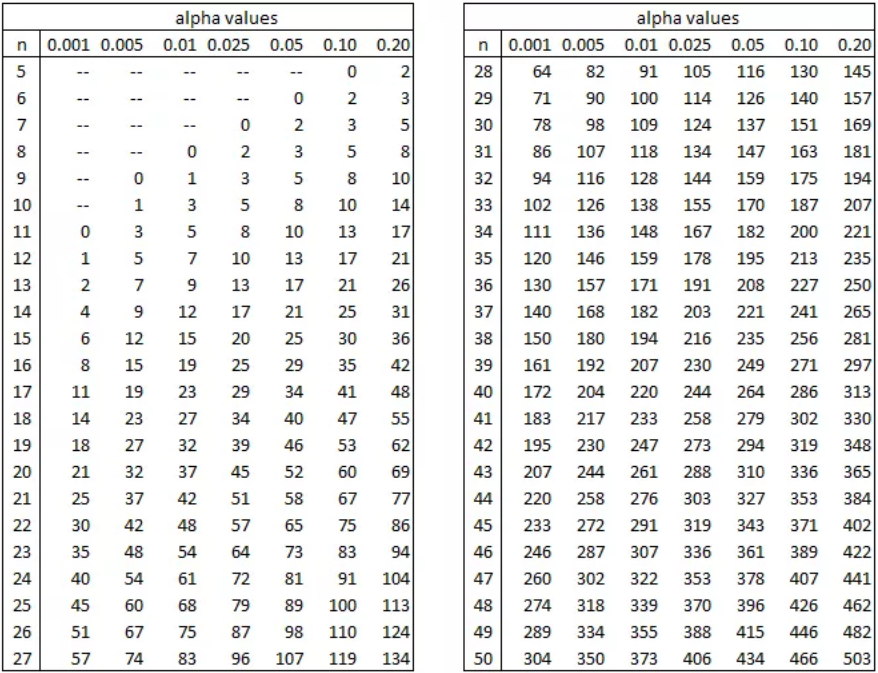
\includegraphics[width=9cm]{./images/signed-rank-test.png}
\end{figure}

\end{frame}


\subsection{Inferences on Proportions}

\begin{frame}{Estimating Proportions}

\justifying
\structb{Proportion.} Let $X_1, \ldots, X_n$ be a random sample of $X$ with sample space $\{0, 1\}$, an unbiased estimator for proportion is given by
\begin{align*}
\widehat{p} = \frac{1}{n}\sum_{i=1}^n X_i.
\end{align*}
\only<1>{
	\begin{itemize}
		\item \underline{Statistic and distribution (by central limit theorem)}.
		\begin{align*}
		Z = \frac{\widehat{p} - p}{\sqrt{p(1-p)/n}} \sim \U{Normal}(0, 1).
		\end{align*}
		\item \underline{$100(1-\alpha)\%$ two-sided confidence interval for $p$}.
		\begin{align*}
		\widehat{p} \pm z_{\alpha/2}\sqrt{\widehat{p}(1-\widehat{p})/n}.
		\end{align*}
	\end{itemize}
}
\only<2>{
	\begin{itemize}
		\item \underline{Choose sample size}. $\widehat{p}$ differs from $p$ by at most $d$ with $100(1-\alpha)\%$ confidence.
		\begin{align*}
		d = z_{\alpha/2}\sqrt{\widehat{p}(1-\widehat{p})/n} \quad \Rightarrow \quad n = \frac{z_{\alpha/2}^2\widehat{p}(1-\widehat{p})}{d^2}.
		\end{align*}
		When no estimate for $p$ is available, we use
		\begin{align*}
		n = \frac{z_{\alpha/2}^2}{4d^2}.
		\end{align*}
	\end{itemize}
}

\end{frame}

\begin{frame}{Hypothesis Testing on Proportion}

\justifying
\structb{Large-sample test for proportion.} Let $X_1, \ldots, X_n$ be a random sample of size $n$ from a Bernoulli distribution with parameter $p$ and let $\widehat{p} = \overline{X}$ denote the sample mean. The test statistic is 
\begin{align*}
Z = \frac{\widehat{p} - p_0}{\sqrt{p_0(1-p_0)/n}}.
\end{align*}
We reject at significance level $\alpha$
\begin{itemize}
	\item $H_0: p = p_0$ if $|Z| > z_{\alpha/2}$,
	\item $H_0: p\leq p_0$ if $Z > z_{\alpha}$,
	\item $H_0: p\geq p_0$ if $Z < -z_{\alpha}$.
\end{itemize}

\end{frame}

\begin{frame}{Comparing Two Proportions}

\justifying
\structb{Difference of proportions.} Suppose we have random samples of sizes $n_1, n_2$ of $X^{(1)}$ and $X^{(2)}$, respectively.
\begin{itemize}
	\item \underline{Statistic and distribution}. For \highlightr{large} sample sizes,
	\begin{align*}
	Z = \frac{\widehat{p}_1 - \widehat{p}_2 - (p_1-p_2)}{\sqrt{\dfrac{p_1(1-p_1)}{n_1} + \dfrac{p_2(1-p_2)}{n_2}}} \sim \U{Normal}(0, 1).
	\end{align*}
	\item \underline{$100(1-\alpha)\%$ two-sided confidence interval for $p_1-p_2$}.
	\begin{align*}
	\widehat{p}_1-\widehat{p}_2 \pm z_{\alpha/2}\sqrt{\dfrac{\widehat{p}_1(1-\widehat{p}_2)}{n_1} + \dfrac{\widehat{p}_2(1-\widehat{p}_2)}{n_2}}.
	\end{align*}
\end{itemize}

\end{frame}

\begin{frame}{Hypothesis Testing on Difference of Proportions}

\justifying
\structb{Test for comparing two proportions.} Let $X_1^{(i)}, \ldots, X_{n_i}^{(i)}, i = 1, 2$ be random samples of sizes $n_i$ from two Bernoulli distributions with parameters $p_i$ and let $\widehat{p}_i = \overline{X}_i$ denote the corresponding sample means. The test statistic is given by
\begin{align*}
Z = \frac{\widehat{p}_1 - \widehat{p}_2 - (p_1-p_2)_0}{\sqrt{\dfrac{\widehat{p}_1(1-\widehat{p}_1)}{n_1} + \dfrac{\widehat{p}_2(1-\widehat{p}_2)}{n_2}}}.
\end{align*}
We reject at significance level $\alpha$
\begin{itemize}
	\item $H_0: p_1-p_2 = (p_1-p_2)_0$ if $|Z| > z_{\alpha/2}$,
	\item $H_0: p_1-p_2 \leq (p_1-p_2)_0$ if $Z > z_{\alpha}$,
	\item $H_0: p_1-p_2 \geq (p_1-p_2)_0$ if $Z < -z_{\alpha}$.
\end{itemize}

\end{frame}


\begin{frame}{Hypothesis Testing on Equality of Proportions}

\justifying
\structb{Pooled test for equality of proportions.} Let $X_1^{(i)}, \ldots, X_{n_i}^{(i)}, i = 1, 2$ be random samples of sizes $n_i$ from two Bernoulli distributions with parameters $p_i$ and let $\widehat{p}_i = \overline{X}_i$ denote the corresponding sample means. The test statistic is given by
\begin{align*}
Z = \frac{\widehat{p}_1 - \widehat{p}_2}{\sqrt{\widehat{p}(1-\widehat{p})\left(\dfrac{1}{n_1} + \dfrac{1}{n_2} \right)}}, \qquad \widehat{p} = \frac{n_1\widehat{p}_1 + n_2\widehat{p}_2}{n_1+n_2}.
\end{align*}
We reject at significance level $\alpha$
\begin{itemize}
	\item $H_0: p_1 = p_2$ if $|Z| > z_{\alpha/2}$,
	\item $H_0: p_1 \leq p_2$ if $Z > z_{\alpha}$,
	\item $H_0: p_1 \geq p_2$ if $Z < -z_{\alpha}$.
\end{itemize}

\end{frame}

\subsection{Comparing Two Variances}

\begin{frame}{Basic Distribution}

\justifying
\structb{The F-distribution.} Let $\chi_{\gamma_1}^2$ and $\chi_{\gamma_2}^2$ be independent chi-squared random variables with $\gamma_1$ and $\gamma_2$ degrees of freedom, respectively. Then the random variable 
\begin{align*}
F_{\gamma_1, \gamma_2} = \frac{\chi_{\gamma_1}^2/\gamma_1}{\chi_{\gamma_2}/\gamma_2}
\end{align*}
follows a \highlightg{F-distribution with $\gamma_1$ and $\gamma_2$ degrees of freedom}, with density function
\begin{align*}
f_{\gamma_1, \gamma_2} = \gamma_1^{\gamma_1/2}\gamma_2^{\gamma_2/2} \frac{\Gamma\left(\frac{\gamma_1 + \gamma_2}{2} \right)}{\Gamma\left(\frac{\gamma_1}{2} \right)\Gamma\left(\frac{\gamma_2}{2} \right)} \frac{x^{\gamma_1/2-1}}{(\gamma_1 x + \gamma_2)^{(\gamma_1 + \gamma_2)/2}}
\end{align*}
for $x\geq 0$ and $f_{\gamma_1, \gamma_2}(x) = 0$ for $x < 0$. Furthermore,
\begin{align*}
P[F_{\red{\gamma_1, \gamma_2}} < x] = P\left[\frac{1}{F_{\red{\gamma_1, \gamma_2}}} > \frac{1}{x} \right] = 1 - P\left[F_{\red{\gamma_2,\gamma_1}} < \frac{1}{x} \right].
\end{align*}

\end{frame}

\begin{frame}{The F-test for Comparing Variances}

\justifying
\structb{F-test.} Let $S_1^2$ and $S_2^2$ be sample variances based on independent random samples of sizes $n_1$ and $n_2$ drawn from normal populations with means $\mu_1$ and $\mu_2$ and variances $\sigma_1^2$ and $\sigma_2^2$, respectively. The test statistic is given by
\begin{align*}
F_{n_1-1,n_2-1} = \frac{S_1^2}{S_2^2}.
\end{align*}
We reject at significance level $\alpha$
\begin{itemize}
	\justifying
	\item $H_0: \sigma_1 \leq \sigma_2$ if $S_1^2/S_2^2 > f_{\alpha, n_1-1, n_2-1}$,
	\item $H_0: \sigma_1 \geq \sigma_2$ if $S_2^2/S_1^2 > f_{\alpha, n_2-1, n_1-1}$,
	\item $H_0: \sigma_1 = \sigma_2$ if $S_1^2/S_2^2 > f_{\alpha/2, n_1-1, n_2-1}$ or $S_2^2/S_1^2 > f_{\alpha/2, n_2-1, n_1-1}$.
\end{itemize}
\structb{OC curve.} The abscissa is defined by
\begin{align*}
\lambda = \frac{\sigma_1}{\sigma_2}.
\end{align*}

\end{frame}
